

% ============================================================
 
\chapter{Results from Calculus}{}{}
\label{app:calculus}
\makeatletter
\renewcommand\thefigure{B-\@arabic\c@figure}%\thechapter.
%
\renewcommand\thetable{B-\@arabic\c@table}%\thechapter.
\makeatother

\index{data analysis!calculus|(} 
\index{calculus|(} 

\Fint{In this appendix, we review some of the results from calculus that
are either needed explicitly in} the main part of the book or are
conceptually sufficiently important when doing data analysis and
mathematical modeling that you should at least be aware that they
\emph{exist}.

Obviously, this appendix cannot replace a class (or two) in beginning
and intermediate calculus, and this is also not the intent. Instead,
this appendix should serve as a reminder of things that you probably
know already. More importantly, the results are presented here in a
slightly different context than usual. Calculus is generally taught
with an eye toward the theoretical development---it has to be, because
the intent is to teach the entire body of knowledge of 
calculus and therefore the theoretical development is most important.
However, for applications you need a different sort of tricks (based
on the same fundamental techniques, of course), and it generally takes
\emph{years} of experience to make out the tricks from the theory.
This appendix assumes that you have seen the theory at least once, so
I am just reminding you of it, but I want to emphasize those
elementary techniques that are most useful in applications of the kind
explained in this book.

This appendix is also intended as somewhat of a teaser: I have
included some results that are particularly interesting, noteworthy,
or fascinating as an invitation for further study.

The structure of this appendix is as follows:
\begin{enumerate}
\item To get a head start, we first look at some common functions and
  their graphs.
\item Then we discuss the core concepts of calculus proper:
  derivative, integral, limit.
\item Next I mention a few practical tricks and techniques that are
  frequently useful.\clearpage

\item Near the end, there is a section on notation and \emph{very}
  basic concepts. \emph{If you start feeling truly confused, check
    here!} (I did not want to start with that section because I'm
  assuming that most readers know this material already.)
\item I conclude with some pointers for further study.
\end{enumerate}

A note for the mathematically fussy: this appendix quite intentionally
eschews much mathematical sophistication. I know that many of the
statements can be made either more general or more precise. But the
way they are worded here is sufficient for my purpose, and I want to
avoid the obscurity that is the by-product of presenting mathematical
statements in their most general form.\vspace*{-5pt}


% ============================================================
\section{Common Functions}

Functions are mappings, which map a real number into another real
number: $f : \mathbb{R} \mapsto \mathbb{R}$. This mapping is always
unique: every input value $x$ is mapped to exactly one result value
$f(x)$. (The converse is not true: many input values may be mapped to
the same result. For example, the mapping $f(x) = 0$, which maps
\emph{all} values to zero, is a valid function.)

More complicated functions are often built up as combinations of
simpler functions. The most important simple functions are powers,
polynomials and rational functions, and trigonometric and exponential
functions.\vspace*{-5pt}

\subsection{Powers}

\index{calculus!powers} 
\index{powers, calculus}
 
The simplest nontrivial function is the \emph{linear} function: \index{linear functions} 
%
\[
f(x) = a x
\]
%
The constant factor $a$ is the \emph{slope}: if $x$ increases by $1$,
then $f(x)$ increases by $a$. Figure~\ref{fig:linear} shows linear
functions with different slopes.

\begin{figure}
  \centerline{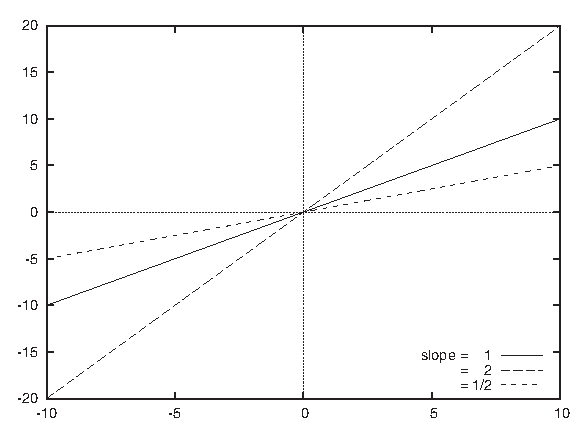
\includegraphics{img/linear}}
  \caption{The linear function $y = ax$.}
  \label{fig:linear}
\end{figure}

The next set of elementary functions are the simple powers:
%
\[
f(x) = x^k
\]
%
The power $k$ can be greater or smaller than $1$. The exponent can be
positive or negative, and it can be an integer or a fraction.  Figure
\ref{fig:powers} shows graphs of some functions with positive integer
powers, and Figure \ref{fig:fracpowers} shows functions with
fractional powers.

\begin{figure}
  \centerline{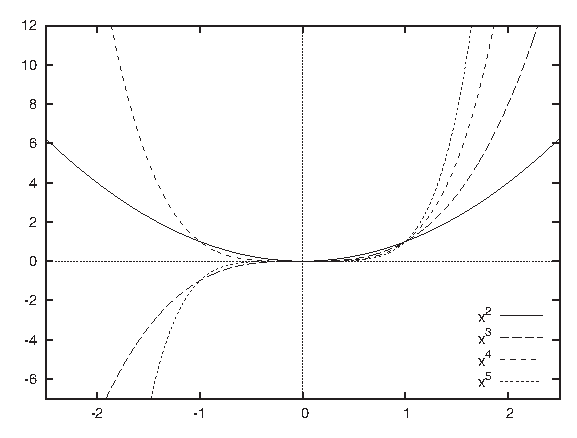
\includegraphics{img/powers}}
  \caption{Simple powers: $y = ax^k$.}
  \label{fig:powers}
\end{figure}

\begin{figure}
  \centerline{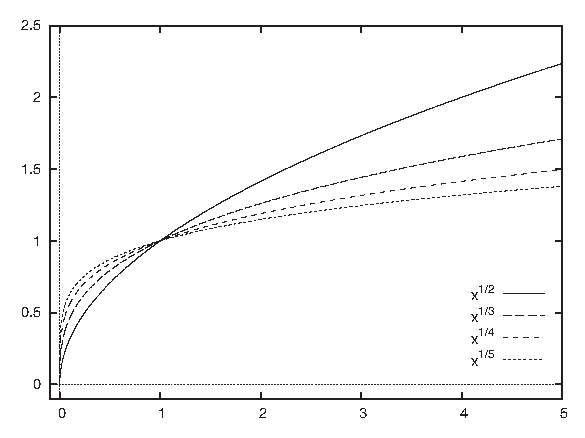
\includegraphics{img/fracpowers}}
  \caption{Fractional powers: $y = a^{p/q}$.}
  \label{fig:fracpowers}\vspace*{-12pt}
\end{figure}

Simple powers have some important properties:

\begin{itemize}
\item All simple powers go through the two points $(0,0)$ and $(1,1)$.
\item The linear function $f(x) = x$ is a simple power with $k = 1$.
\item The square-root function $f(x) = \sqrt{x}$ is a simple power with
  $k = 1/2$.
\item Integer powers ($k=1,2,3,\dotsc$) can be evaluated for negative
  $x$, but for fractional powers we have to be more careful.
\end{itemize}

Powers obey the following laws:
%
\begin{gather*}
x^n x^m = x^{n+m} \\
x^n x^{-m} = \frac{x^n}{x^m} \\
x^0 = 1 \\
x^1 = x
\end{gather*}
%
If the exponent is negative, it turns the expression into a
\emph{fraction}:
%
\[
x^{-n} = \frac{1}{x^n}
\]
%
When dealing with fractions, we must always remember that the
denominator must not become zero. As the denominator of a fraction
approaches zero, the value of the overall expression goes to infinity.
We say: the expression \emph{diverges} and the function has a
\emph{singularity} at the position where the denominator vanishes.
Figure \ref{fig:negpowers} shows graphs of functions with negative
powers.  Note the divergence for $x=0$.\vspace*{-6pt}

\begin{figure}
  \centerline{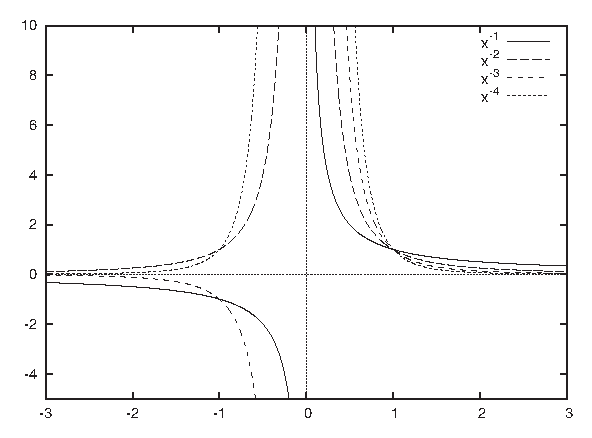
\includegraphics{img/negpowers}}
  \caption{Negative powers: $y = ax^{-k} = a/x^k$.}
  \label{fig:negpowers} \vspace*{9pt}
\end{figure}
    
\subsection{Polynomials and Rational Functions}

\index{calculus!polynomials} 
\index{polynomials!about} 
\index{calculus!rational functions} 
\index{rational functions} 

Polynomials are sums of integer powers together with constant
coefficients:\vspace*{-3pt}
%
\[
p(x) = a_n x^n + a_{n-1} x^{n-1} + \dots + a_2 x^2 + a_1 x + a_0
\]
%
Polynomials are nice because they are extremely easy to handle
mathematically (after all, they are just sums of simple integer
powers).  Yet, more complicated functions can be approximated very
well using polynomials. Polynomials therefore play an important role
as approximations of more complicated functions.

All polynomials exhibit some ``wiggles'' and eventually diverge as $x$
goes to plus or minus infinity (see Figure \ref{fig:polynomial}). The
highest power occurring in a polynomial is known as that \emph{degree}
of the\vadjust{\pagebreak} polynomial.

\begin{figure}
  \centerline{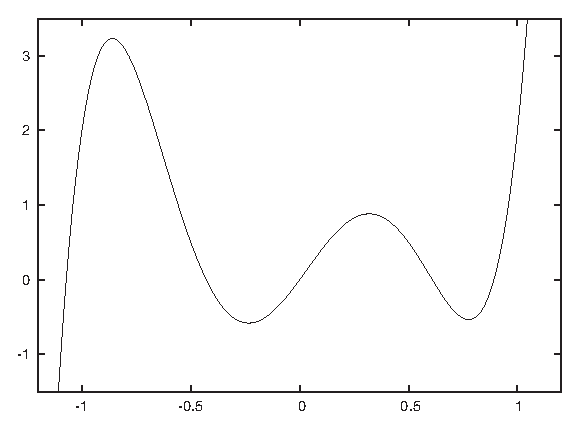
\includegraphics{img/polynomial}}
  \caption{A polynomial: $y = 16 x^5 - 20 x^3 + 2 x^2 + 4 x$.}
  \label{fig:polynomial}\vspace*{-9pt}
\end{figure} 

Rational functions are fractions that have polynomials in both the
numerator and the denominator:
%
\[
r(x) = \frac{p(x)}{q(x)} 
     = \frac{a_n x^n + a_{n-1} x^{n-1} + \dots + a_2 x^2 + a_1 x + a_0}
            {b_m x^m + b_{m-1} x^{m-1} + \dots + b_2 x^2 + b_1 x + b_0}
\]
%
Although they may appear equally harmless, rational functions are
entirely more complicated beasts than polynomials. Whenever the
denominator becomes zero, they blow up. The behavior as $x$ approaches
infinity depends on the relative size of the largest powers in
numerator and denominator, respectively. Rational functions are
\emph{not} simple functions.
    
\subsection{Exponential Function and Logarithm}

\index{calculus!exponential functions|(} 
\index{exponential function|(} 
\index{calculus!logarithms|(} 
\index{logarithms!calculus|(} 

Some functions cannot be expressed as polynomials (or as fraction of
polynomials) of finite degree. Such functions are known as
\emph{transcendental functions}. \index{transcendental functions} For our purposes, the most important
ones are the exponential function $f(x) = e^x$ (where $e =
2.718281\dots$ is Euler's number) and its inverse, the logarithm.

A graph of the exponential function is shown in Figure
\ref{fig:exponential}. For positive argument the exponential function
grows \emph{very} quickly, and for negative argument it decays equally
quickly. The exponential function plays a central role in growth and
decay processes.

\begin{figure}
  \centerline{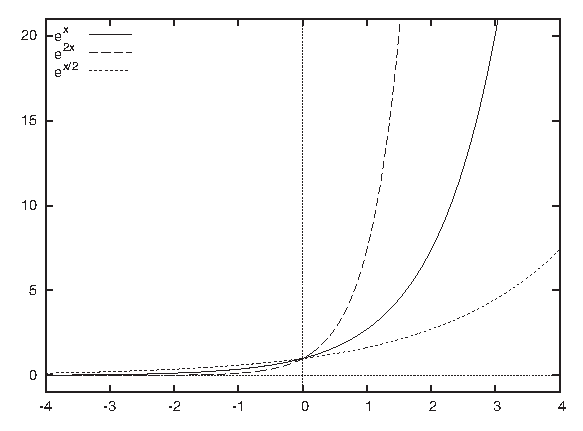
\includegraphics{img/exponential}}
  \caption{The exponential function $y = e^x$.}
  \label{fig:exponential}\vspace*{-9pt}
\end{figure}
  
Some properties of the exponential function follow from the rules for
powers:
%
\begin{gather*}
  e^x \, e^y = e^{x+y} \\
  e^{-x} = \frac{1}{e^x}
\end{gather*}
%

The logarithm is the inverse of the exponential function; in other
words:
%
\begin{gather*}
  y = e^x \quad \iff \quad \log y = x \\
  e^{\log(x)} = x \quad \text{and} \quad \log\paren{ e^x } = x
\end{gather*}

A plot of the logarithm is shown in Figure \ref{fig:logarithm}. The
logarithm is defined only for strictly positive values of $x$, and it
tends to negative infinity as $x$ approaches zero. In the opposite
direction, as $x$ becomes large the logarithm grows without bounds,
but it grows almost unbelievably slowly. For $x=2$, we have $\log 2 =
0.69\dots$ and for $x=10$ we find $\log 10 = 2.30\dots$, but for
$x=\text{1,000}$ and $x=10^6$ we have only $\log 1000 = 6.91\dots$ and
$\log 10^6 = 13.81\dots$, respectively. Yet the logarithm does not
have an upper bound: it keeps on growing but at an ever-decreasing
rate of growth.

\begin{figure}
  \centerline{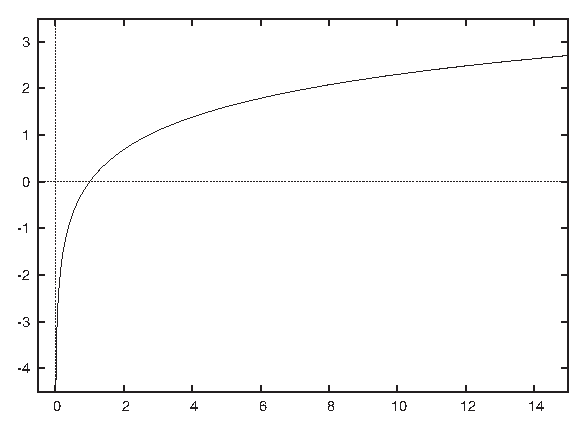
\includegraphics{img/logarithm}}
  \caption{The natural logarithm: $y = \log(x)$.}
  \label{fig:logarithm}
\end{figure}

The logarithm has a number of basic properties:
%
\begin{gather*}
\log( 1 ) = 0 \\
\log( x \, y ) = \log x + \log y \\
\log( x^k ) = k \, \log x
\end{gather*}
%
As you can see, logarithms turn products into sums and powers into
products. In other words, logarithms ``simplify'' expressions. This
property was (and is!) used in numerical calculations: instead of
multiplying two numbers (which is complicated), you add their
logarithms (which is easy---provided you have a logarithm table or a
slide rule) and then exponentiate the result. This calculational
scheme is still relevant today, but not for the kinds of simple
products that previous generations performed using slide rules.
Instead, logarithmic multiplication can be necessary when dealing with
products that would generate intermediate over- or underflows even
though the final result may be of reasonable size. In particular,
certain kinds of combinatorial and probabilistic problems require
finding the maximum of expressions such as $p^n (1-p)^k$, where $p<1$
is a probability and $n$ and $k$ may be\vadjust{\pagebreak} large numbers. Brute-force
evaluation will underflow even for modest values of the exponents, but
taking logarithms first will result in a numerically harmless
expression.

\index{calculus!exponential functions|)} 
\index{exponential function|)} 
\index{calculus!logarithms|)} 
\index{logarithms!calculus|)} 
    
\subsection{Trigonometric Functions}

\index{calculus!trigonometric functions} 
\index{trigonometric functions} 

The trigonometric functions describe oscillations of all kinds and
thus play a central role in sciences and engineering. Like the
exponential function, they are transcendental functions, meaning they
cannot be written down as a polynomial of finite degree.

Figure \ref{fig:trigonometrics} shows graphs of the two most important
trigonometric functions: $\sin(x)$ and $\cos(x)$. The cosine is equal
to the sine but is shifted by $\pi/2$ (90 degrees) to the left. We
can see that both functions are \emph{periodic}: they repeat themselves
\emph{exactly} after a period of length $2\pi$. In other words, $\sin(x
+ 2\pi) = \sin(x)$ and $\cos(x + 2\pi) = \cos(x)$.

\begin{figure}
  \centerline{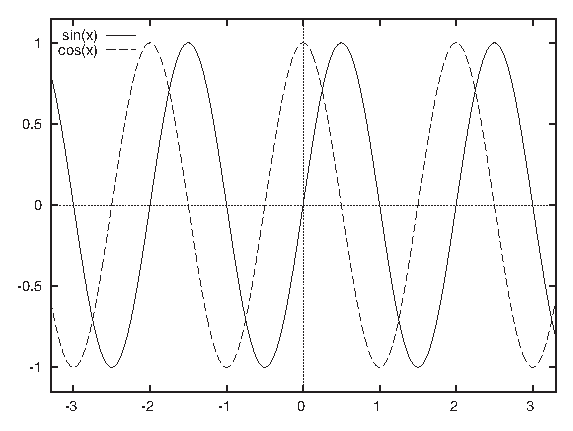
\includegraphics{img/trig}}
  \caption{The trigonometric functions $\sin(x)$ and $\cos(x)$.}
  \label{fig:trigonometrics}
\end{figure}

The length of the period is $2\pi$, which you may recall is the
\emph{circumference of a circle with radius equal to $1$}. This should
make sense, because $\sin(x)$ and $\cos(x)$ repeat themselves after
advancing by $2\pi$ and so does  the circle: if you go around the
circle once, you are back to where you started. This similarity
between the trigonometric functions and the geometry of the circle is
no accident, but this is not the place to explore it.

Besides their periodicity, the trigonometric functions obey a number
of rules and properties (``trig identities''), only one of which 
is important enough to mention here:
%
\[
\sin^2 x + \cos^2 x = 1 \quad \text{for all $x$}
\]
%
Finally, I should mention the tangent function, which is occasionally
useful:
%
\[
\tan x = \frac{\sin(x)}{\cos(x)}
\]
%    

\subsection{Gaussian Function and the Normal Distribution}

\index{calculus!Gaussian function and the Normal distribution} 
\index{Gaussian distribution (Gaussian function)!about} 

The Gaussian function arises frequently and in many different
contexts. It is given by the formula:
%
\[
\phi(x) = \frac{1}{\sqrt{2 \pi}} e^{-\frac{1}{2}x^2}
\]
%
and its plot is shown in Figure \ref{fig:gausspdf}. (This is the form
in which the Gaussian should be memorized, with the factor $1/2$ in
the exponent and the factor $1/\sqrt{2\pi}$ up front: they ensure that
the integral of the Gaussian over all $x$ will be equal to $1$.)

\begin{figure}
  \centerline{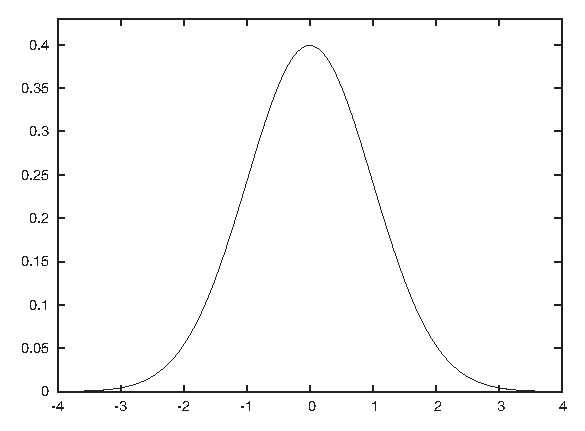
\includegraphics{img/gausspdf}}
  \caption{The Gaussian: 
    $y = \frac{1}{\sqrt{2 \pi}} e^{-\frac{1}{2}x^2}$.}
  \label{fig:gausspdf} 
\end{figure} 

Two applications of the Gaussian stand out. First of all, a strong
result from probability theory, the \emph{Central Limit Theorem}\index{Central Limit Theorem!Gaussian distribution} 
states that (under rather weak assumptions) if we add many random
quantities, then their sum will be distributed according to a Gaussian
distribution. In particular, if we take several samples from a
population and calculate the mean for each sample, then the sample
means will be distributed according to a Gaussian. Because of this,
the Gaussian arises \emph{all the time} in probability theory and
statistics.

It is because of this connection that the Gaussian is often identified
as ``the'' bell curve---quite incorrectly so, since there are many
bell-shaped curves, many of which have drastically different\vadjust{\pagebreak}
properties. In fact, there are important cases where the Central Limit
Theorem fails, and the Gaussian is \emph{not} a good way to describe
the behavior of a random system (see the discussion of power-law
distributions in Chapter \ref{ch:probability}).

The other context in which the Gaussian arises frequently is as a
\emph{kernel}---that is, as a strongly peaked and localized yet very
smooth function. Although the Gaussian is greater than zero
everywhere, it falls off to zero so quickly that almost the entire
area underneath it is concentrated on the interval $-3 \le x \le 3$.
It is this last property that makes the Gaussian so convenient to use
as a kernel.  Although the Gaussian is defined and nonzero everywhere
(so that we don't need to worry about limits of integration), it can
be multiplied against almost any function and integrated. The integral
will retain only those values of the function near zero; values at
positions far from the origin will be suppressed (smoothly) by the
Gaussian.

In statistical applications, we are often interested in the area under
certain parts of the curve because that will provide the answer to
questions such as: ``What is the probability that the point lies
between $-1$ and $1$?''  The antiderivative of the Gaussian cannot be
expressed in terms of elementary functions; instead it is defined
through the integral directly:
%
\[
\Phi(x) = 
  \frac{1}{\sqrt{2 \pi}} 
  \int_{-\infty}^x \! e^{-\frac{1}{2} t^2} \rms{t}
\]
%
This function is known as the \emph{Normal distribution function}\index{Normal distribution function}\index{Gaussian distribution function} 
(see Figure \ref{fig:gausscdf}). As previously mentioned, the factor
$1/\sqrt{2 \pi}$ is a normalization constant that ensures the area
under the entire curve is $1$.

\begin{figure}
  \centerline{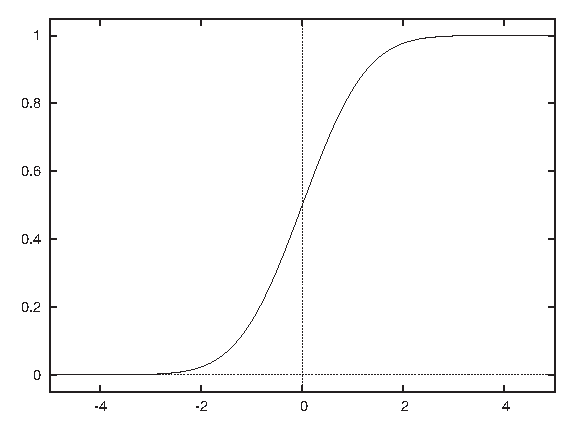
\includegraphics{img/gausscdf}}
  \caption{The Gaussian distribution function.}
  \label{fig:gausscdf}
\end{figure}

Given the function $\Phi(x)$, a question like the one just given can
be answered easily: the area over the interval $[-1,1]$ is simply
$\Phi(1) - \Phi(-1)$.

\subsection{Other Functions}

There are some other functions that appear in applications often
enough that we should be familiar with them but are a bit more exotic
than the families of functions considered so far.

\begin{figure}
  \centerline{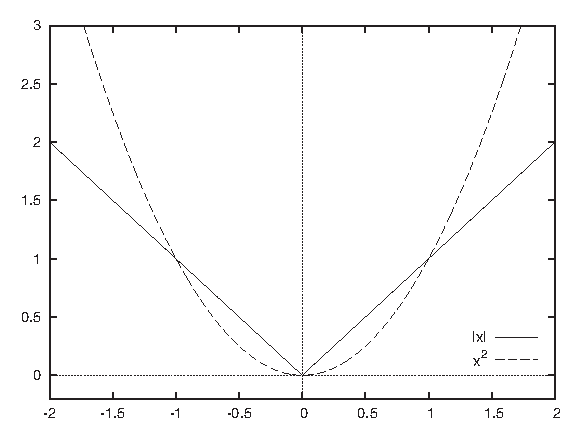
\includegraphics{img/absvalue}}
  \caption{The absolute value function $y = \abs{x}$ and the square $y
    = x^2$.}
  \label{fig:absvalue}
\end{figure} 

The \emph{absolute value} function is defined as:\index{calculus!absolute value function}\index{absolute value function} 
%
\[
|a| = 
\begin{cases} 
  \enskip a & \text{if $a \ge 0$} \\
  -a & \text{otherwise}
\end{cases}
\]
%
In other words, it is the positive (``absolute'') value of its
argument. From a mathematical perspective, the absolute value is hard
to work with because of the need to treat the two possible cases
separately and because of the kink at $x=0$, which poses difficulties
when doing analytical work.  For this reason, one instead often uses
the square $x^2$ to guarantee a positive value.  The square relieves
us of the need to worry about special cases explicitly, and it is
smooth throughout. However, the square is relatively smaller than the
absolute value for small values of $x$ but relatively larger for large
values of $x$. Weight functions \index{weight functions} based on the square (as in
least-squares methods, for instance) therefore tend to overemphasize
outliers (see Figure \ref{fig:absvalue}).



Both the \emph{hyperbolic tangent} $\tanh(x)$ (pronounced: tan-sh) and\index{calculus!hyperbolic tangent function}\index{hyperbolic tangent function} 
the \emph{logistic function} are S-shaped or sigmoidal functions. The
latter function is the solution to the \emph{logistic differential
  equation}, hence the name. The logistic\vadjust{\pagebreak} differential equation is
used to model constrained growth processes such as bacteria competing
for food and infection rates for contagious diseases. Both these
functions are defined in terms of the exponential functions as
follows:
%
\begin{gather*}
  \tanh(x)            = \frac{e^x - e^{-x}}{e^x + e^{-x}} \\
  \operatorname{P}(x) = \frac{1}{1 + e^{-x}}
\end{gather*}
%
Both functions are smooth approximations to a step function, and they
differ mostly in the range of values they assume: the $\tanh(x)$ takes on
values in the interval $[-1,1]$, whereas the logistic function takes
on only positive values between $0$ and $1$ (see Figure
\ref{fig:sigmoid}). It is not hard to show that the two functions can
be transformed into each other; in fact, we have $\operatorname{P}(x)
= (\tanh(x/2)+1)/2$.

\begin{figure}
  \centerline{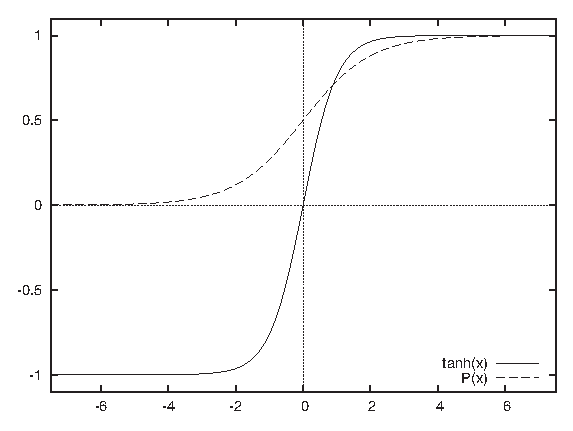
\includegraphics{img/step}}
  \caption{Two sigmoid (step) functions: the hyperbolic tangent $y =
    \tanh(x)$ and the logistic function $y = 1/(1 + e^{-x})$.}
  \label{fig:sigmoid}
\end{figure}

These two functions are each occasionally referred to as \emph{the}
sigmoid function. \index{sigmoid function} That is incorrect: there are infinitely many
functions that smoothly interpolate a step function. But among those
functions, the two discussed here have the advantage that---although
everywhere smooth---they basically consist of three straight lines:
very flat as $x$ goes to plus or minus infinity and almost linear in
the transition regime. The position and steepness of the transition
can be changed through a standard variable transformation; for
example, $\tanh( (x-m)/a )$ will have a transition at $m$ with local
slope $1/a$.

The last function to consider here is the \emph{factorial}: $n!$.\index{calculus!factorial function}\index{factorial function}\index{factorial function} The
factorial is defined only for nonnegative integers, as follows:
%
\begin{align*}
  0! & = 1 \\
  n! & = 1 \cdot 2 \cdot \dots \cdot (n-1) \cdot n
\end{align*}
%
The factorial plays an important role in combinatorial problems, since
it is the number of ways that $n$ distinguishable objects can be
arranged. (To see this, imagine that you have to fill $n$ boxes with
$n$ items. To fill the first box, you have $n$ choices. To fill the
second box, you have $n-1$ choices. And so on. The total number of
arrangements or \emph{permutations} is therefore $n \cdot (n-1) \dotsb
1 = n!$.)

The factorial grows \emph{very} quickly; it grows faster even than the
exponential. Because the
factorial grows so quickly, it is often convenient to work with its
logarithm.  An important and widely used approximation for the
logarithm of the factorial is \emph{Stirling's approximation}:
%
\[
\log n! \approx n \log(n) - n \qquad \text{for large $n$}
\]
%
For the curious: it is possible to define a function that smoothly
interpolates the factorial for all positive numbers (not just
integers). It is known as the \emph{Gamma function}, and it is another
example (besides the Gaussian distribution function) for a function
defined through an integral:
%
\[
\Gamma(x) = \int_0^\infty \! t^{x-1} e^{-t} \rms{t}
\]
%
The variable $t$ in this expression is just a ``dummy'' variable of
integration---it does not appear in the final result. You can see
that the first term in the integral grows as a power while the
second falls exponentially, with the effect that the value of the
integral is finite. Note that the limits of integration are fixed. The
independent variable $x$ enters the expression only as a parameter.
Finally, it is easy to show that the Gamma function obeys the rule $n
\, \Gamma(n) = \Gamma(n+1)$, which is the defining property of the
factorial function.

We do not need the Gamma function in this book, but it is interesting
as an example of how integrals can be used to define and construct new
functions.

\subsection{The Inverse of a Function}

\index{calculus!inverse of a function} 
\index{inverse of a function} 

A function maps its argument to a result: given a value for $x$, we
can find the corresponding value of $f(x)$. Occasionally, we want to
turn this relation around and ask: given a value of $f(x)$, what is
the corresponding value of $x$? 

That's what the \emph{inverse function} does: if $f(x)$ is some
function, then its inverse $f^{-1}(x)$ is defined as the function
that, when applied to $f(x)$, returns the original argument:
%
\[
f^{-1}\paren{ f(x) } = x
\]
%

Sometimes we can invert a function explicitly. For example, if $f(x) =
x^2$, then the inverse function is the square root, because $\sqrt{
  x^2 } = x$ (which is the definition of the inverse function).  In a
similar way, the logarithm is the inverse function of the exponential:
$\log( e^x ) = x$.

In other cases, it may not be possible to find an explicit form for
the inverse function. For example, we sometimes need the inverse of
the Gaussian distribution function $\Phi(x)$. However, no simple form
for this function exists, so we write it symbolically as
$\Phi^{-1}(x)$, which refers to the function for which
$\Phi^{-1}\paren{ \Phi(x) } = x$ is true.


% ============================================================
\section{Calculus}

Calculus proper deals with the consideration of limit processes: how
does a sequence of values behave if we make infinitely many steps? 
The slope of a function and the area underneath a function are both
defined through such limit processes (the derivative and the integral,
respectively).

Calculus allows us to make statements about properties of functions
and also to develop approximations.

\begin{figure}
  \centerline{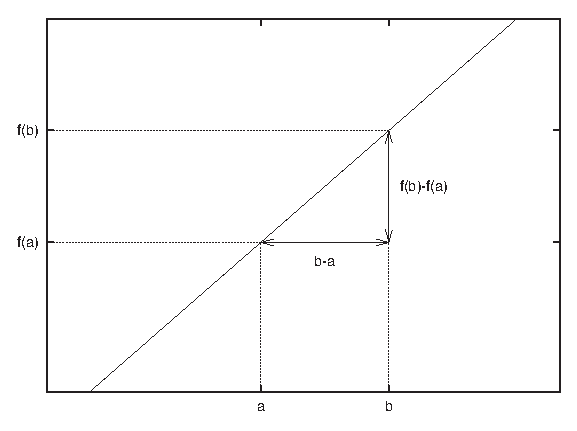
\includegraphics{img/linslope}}
  \caption{The slope of a linear function is the ratio of the growth
    in the vertical direction, $f(b)-f(a)$, divided by the
    corresponding growth in the horizontal direction, $b-a$.}
  \label{fig:linslope}\vspace*{-9pt}
\end{figure}

% --------------------------------------------------  
\subsection{Derivatives}

\index{calculus!derivatives|(} 
\index{derivatives|(} 

We already mentioned the slope as the rate of change of a linear
function. The same concept can be extended to nonlinear functions,
though for such functions, the slope itself will vary from place to
place. For this reason, we speak of the \emph{local slope} of a
curve at each point.

Let's examine the slope as the \emph{rate of change} of a function in
more detail, because this concept is of fundamental importance
whenever we want to interpolate or approximate some data by a smooth
function. Figure \ref{fig:linslope} shows the\vadjust{\pagebreak} construction used to
calculate the slope of a linear function. As $x$ goes from $a$ to $b$,
the function changes from $f(a)$ to $f(b)$. The rate of change is the
ratio of the change in $f(x)$ to the change in $x$:
%
\[
\text{slope} = \frac{f(b) - f(a)}{b - a}
\]
%
Make sure that you really understand this formula!



Now, let's apply this concept to a function that is nonlinear.
Because the slope of the curve varies from point to point, we cannot
find the slope directly using the previous formula; however, we can
use the formula to \emph{approximate} the local slope.

Figure \ref{fig:derivative} demonstrates the concept. We fix two
points on a curve and put a straight line through them. This line has
a slope, which is $\frac{f(b) - f(a)}{b - a}$. This is only an
approximation to the slope at point $a$.  But we can improve the
approximation by moving the second point $b$ closer to $a$. If we let
$b$ go all the way to $a$, we end up with the (local) slope \emph{at}
the point $a$ exactly. This is called the \emph{derivative}.  (It is a
central result of calculus that, although numerator and denominator in
$\frac{f(b) - f(a)}{b - a}$ each go to zero separately in this
process, the fraction itself goes to a well-defined value.)

\begin{figure}
  \centerline{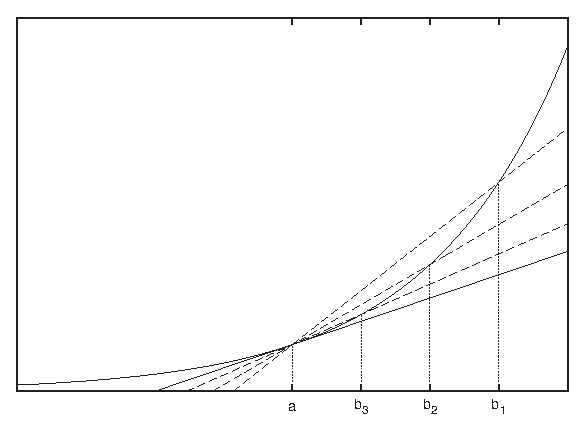
\includegraphics{img/derivative}}
  \caption{As $b_i$ approaches $a$, the slope found for these two
    points becomes closer and closer to the local\hfill\break slope at $a$.}
  \label{fig:derivative}\vspace*{-9pt}
\end{figure}

The construction just performed was done graphically and for a single
point only, but it can be carried out analytically in a fully general
way. The process is sufficiently instructive that we shall study a
simple example in detail---namely finding a general rule for the
derivative of the function $f(x) = x^2$. It will be useful to rewrite
the\vadjust{\pagebreak} interval $[a,b]$ as $[x, x+\epsilon]$. We can now go ahead and
form the familiar ratio:
%
\begin{align*}
\frac{ f(b) - f(a) }{ b - a } 
 & = \frac{ f(x+\epsilon) - f(x)}{ (x+\epsilon) - x } \\
 & = \frac{(x+\epsilon)^2 - x^2}{x+\epsilon - x} \\
 & = \frac{x^2 + 2x\epsilon + \epsilon^2 - x^2}{\epsilon} \\
 & = \frac{2x\epsilon + \epsilon^2}{\epsilon} \\
 & = 2x + \epsilon \\
 & \to 2x \quad \text{as $\epsilon$ goes to zero}
\end{align*}
%
In the second step, the terms not depending on $\epsilon$ cancel each
other; in the third step, we cancel an $\epsilon$ between the
numerator and the denominator, which leaves an expression that is
perfectly harmless as $\epsilon$ goes to zero! The (harmless) result
is the sought-for derivative of the function. Notice that the result
is true for \emph{any} $x$, so we have obtained an expression for the
derivative of $x^2$ that holds for all $x$: the derivative of $x^2$ is
$2x$. Always. Similar rules can be set up for other functions (you may
try your hand at finding the rule for $x^3$ or even $x^k$ for general
$k$).  Table \ref{tbl:derivatives} lists a few of the most important
ones.

There are two ways to indicate the derivative. A short form uses the
prime, like this: $f^\prime(x$) is the derivative of $f(x)$. Another
form uses the \emph{differential operator} $\frac{\rm d}{{\rm d}x}$, %$\displaystyle\diff{}{  x}$, 
which acts on
the expression to its right. Using the latter, we can write:
%
\[
\Diff{x} x^2 = 2x
\]
%

\begin{table}
\def\vrl{\smash{\vrule height64pt width.25pt depth4pt}}
\tabcolsep12pt
\tbl{Derivatives and antiderivatives (integrals) for a few 
  elementary functions.\label{tbl:derivatives}}{%
\begin{tabular}{c@{\hskip9pt}c@{\hskip9pt}c@{\hskip9pt}c@{\hskip9pt}c}\toprule
\TCH{Function} & & \TCH{Derivative} && \TCH{Integral} \\\colrule
$ x^n $ && $ n x^{n-1} $ && $ \frac{1}{n+1} x^{n+1} $  \\
$ e^x $ && $ e^x $ && $ e^x $ \\
$ \log x $ && $ 1/x $ && $ x \log x - x $ \\
$ \sin x $ && $ \cos x $ && $ -\cos x $ \\
$ \cos x $ &\vrl& $ -\sin x $ &\vrl& $ \sin x $ \\
\end{tabular}}
\end{table}

% $ f(x) + g(x) $ & $ f^\prime(x) + g^\prime(x) $ & \\
% $ f(x) \, g(x) $ & $ f^\prime(x) \, g(x) + f(x) \, g^\prime(x) $ & \\
% $ f( g(x) ) $ & $ f^\prime( g(x) ) \, g^\prime(x) $ & \\

\index{calculus!derivatives|)} 
\index{derivatives|)} 

% --------------------------------------------------  
\subsection{Finding Minima and Maxima}

\index{calculus!minima and maxima} 
\index{minima and maxima, functions} 

When a smooth function reaches a local minimum or maximum, its slope
at that point is zero. This is easy to see: as you approach a peak,
you go uphill (positive slope); once over the top, you go downhill
(negative slope). Hence, you must have passed a point where you were
going neither uphill nor downhill---in other words, where the slope
was zero. (From a mathematically rigorous point of view, this is not
quite as obvious as it may seem; you may want to check for ``Rolle's
theorem'' in a calculus text.)

The opposite is also true: if the slope (\ie, the derivative) is zero
somewhere, then the function has either a minimum or a maximum at that
position. (There is also a third possibility: the function has a
so-called saddle point there. In practice, this occurs less
frequently.) Figure \ref{fig:minmaxsaddle} demonstrates all these
cases.

\begin{figure}
  \centerline{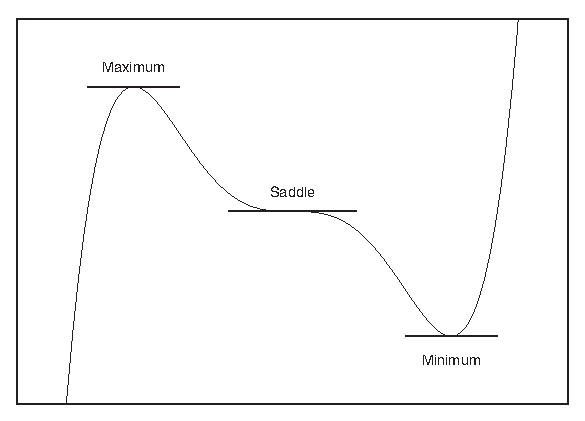
\includegraphics{img/minmaxsaddle}}
  \caption{The slope of a curve is zero when the curve reaches a
    maximum, a minimum, or a saddle point. Zeros in the derivative
    therefore indicate the occurrence of one of those special points.}
  \label{fig:minmaxsaddle}\vspace*{-9pt}
\end{figure} 

We can therefore use derivatives to locate minima or maxima of a
function. First we determine the derivative of the function, and then
we find the locations where the derivative is zero (the derivative's
\emph{roots}). The roots are the locations of the extrema of the
original function.

Extrema \index{extrema} are important because they are the solution to
\emph{optimization} problems. \index{optimization problems!extrema} Whenever we want to find the ``best''
solution in some context, we are looking for an extremum: the lowest
price, the longest duration, the greatest utilization, the highest
efficiency. Hence, if we have a mathematical expression for the price,
duration, utilization, or efficiency, we can take its derivative with
respect to its parameters, set the derivative to zero, and solve for
those values of the parameters that maximize (or minimize) our
objective function.\vspace*{-6pt}

% NEED AN EXAMPLE INVOLVING A COST-BENEFIT TRADE-OFF HERE! 
    
% --------------------------------------------------  
\subsection{Integrals}

\index{calculus!integrals} 
\index{integrals!about} 

\looseness-1Derivatives find the local rate of change of a curve as the limit of a
sequence of better and better approximations. Integrals calculate the
area underneath a curve by a similar method.

Figure \ref{fig:integral} demonstrates the process. We approximate the
area underneath a curve by using rectangular boxes. As we make the
boxes narrower, the approximation becomes more accurate.  In the limit
of infinitely many boxes of infinitely narrow width, we obtain the exact
area under the curve.

\begin{figure}
  \centerline{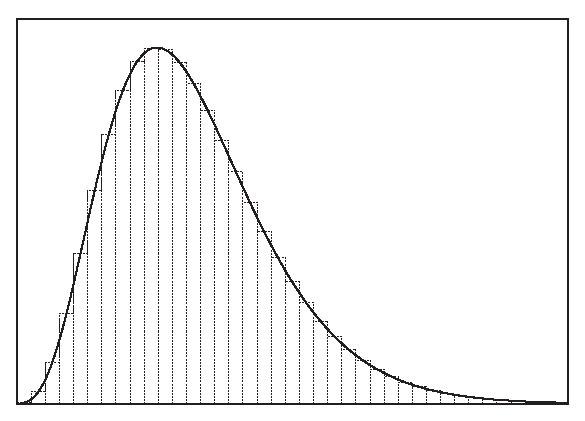
\includegraphics{img/integral}}
  \caption{The integral is the area under a curve. It can be
    approximated by filling the area under the curve with narrow
    rectangles and adding up their areas.  The approximation improves
    as the width of the rectangles becomes smaller.}
  \label{fig:integral}
\end{figure}\pagebreak

Integrals are conceptually very simple but analytically much more
difficult than derivatives. It is always possible to find a
closed-form expression for the derivative of a function. This is not
so for integrals in general, but for some simple functions an
expression for the integral can be found. Some examples are included
in Table \ref{tbl:derivatives}.

Integrals are often denoted using uppercase letters, and there is a
special symbol to indicate the ``summing'' of the area underneath a
curve:
%
\[
F(y) = \int f(x) \rms{x}
\]
%
We can include the limits of the domain over which we want to
integrate, like this:
%
\[
A = \int_a^b f(x) \rms{x}
\]
%
Notice that $A$ is a \emph{number}, namely the area underneath the
curve between $x=a$ and $x=b$, whereas the indefinite integral
(without the limits) is a \emph{function}, which can be evaluated at
any point.
  
% --------------------------------------------------  
\subsection{Limits, Sequences, and Series}

\index{calculus!limits, sequences and series}
\index{limits, calculus}
\index{sequences, calculus}   
\index{series, calculus} 

The central concept in all of calculus is the notion of a
\emph{limit}. The basic idea is as follows. We construct some process
that continues indefinitely and approximates some value ever more
closely as the process goes on---but without reaching the limit in any
finite number of steps, no matter how many. The important insight is
that, even though the limit is never reached, we can nevertheless make
statements about the limiting value. The derivative (as the limit of
the difference ratio) and the integral (as the limit of the sum of
approximating ``boxes'') are examples that we have already
encountered.

As simpler example, consider the numbers $1/1$, $1/2$, $1/3$, $1/4$,
$\dots$ or $1/n$ in general as $n$ goes to infinity. Clearly, the
numbers approach zero ever more closely; nonetheless, for any finite
$n$, the value of $1/n$ is always greater than zero. We call such an
infinite, ordered set of numbers a \emph{sequence}, and zero is the
limit of this particular sequence.

A \emph{series} is a sum:
%
\begin{align*}
s_n & = \sum_{i=0}^n a_n \\
    & = a_0 + a_1 + a_2 + a_3 + \dots + a_n
\end{align*}
%
As long as the number of terms in the series is finite, there is no
problem. But once we let the number of terms go to infinity, we need
to ask whether the sum still converges to a finite value. We have
already seen a case where it does: we defined the integral as the
value of the infinite sum of infinitely small boxes.

It may be surprising that an \emph{infinite} sum can still add up to a
\emph{finite} value. Yet this can happen provided the terms in the sum
become smaller rapidly enough. Here's an example: if you sum up 1,
0.1, 0.01, 0.001, 0.0001, \dots, you can see that the sum approaches
$1.1111\dotsc$ but will never be larger than 1.2.  Here is a more
dramatic example: I have a piece of chocolate. I break it into two
equal parts and give you one. Now I repeat the process with what I
have left, and so on. Obviously, we can continue like this forever
because I always retain half of what I had before. However, you will
never accumulate more chocolate than what I started out with!

An infinite series converges to a finite value only if the magnitude
of the terms decreases sufficiently quickly. If the terms do not become
smaller fast enough, the series diverges (\ie, its value is infinite).
An important series that does \emph{not} converge is the
\emph{harmonic series}:
%
\[
\sum_{k=1}^\infty \frac{1}{k} 
= 1 + \frac{1}{2} + \frac{1}{3} + \dots = \infty
\]
%
One can work out rigorous tests to determine whether or not a given
series converges. For example, we can compare the terms of the series
to those from a series that is known to converge: if the terms in the
new series become smaller more quickly than in the converging series,
then the new series will also converge.

Finding the value of an infinite sum is often tricky, but there is one
example that is rather straightforward. The solution involves a trick
well worth knowing. Consider the infinite \emph{geometric series}:
%
\[
s = \sum_{i=0}^{\infty} = 1 + q + q^2 + q^3 + \dotsb \qquad \text{for $|q| < 1$}
\]
%
Now, let's multiply by $q$ and add 1:
\begin{align*}
q s + 1 & = q ( 1 + q + q^2 + q^3 + \dotsb ) + 1 \\
        & = q + q^2 + q^3 + q^4 + \dots + 1 \\
        & = s
\end{align*}
%
To understand the last step, realize that the righthand side equals
our earlier definition of $s$. We can now solve the resulting equation
for $s$ and obtain:
%
\[
s = \frac{1}{1-q}
\]
%
This is a good trick that can be applied in similar cases: if you can
express an infinite series in terms of itself, the result may be an
equation that you can solve explicitly for the unknown value of the
infinite series.


% --------------------------------------------------  
\subsection{Power Series and Taylor Expansion}

\index{calculus!power series and Taylor expansion} 
\index{power series and Taylor expansion} 
\index{Taylor expansion} 

An especially important kind of series contains consecutive powers of
the variable $x$ multiplied by the constant coefficients $a_i$.  Such
series are called \emph{power series}. The variable $x$ can take on
any value (it is a ``dummy variable''), and the sum of the series is
therefore a function of $x$:
%
\[
s(x) = \sum_{i=0}^n a_i x^i
\]
%
If $n$ is finite, then there is only a finite number of terms in the
series: in fact, the series is simply a polynomial (and, conversely,
every polynomial is a finite power series). But the number of terms
can also be infinite, in which case we have to ask for what values of
$x$ does the series converge. Infinite power series are of great
theoretical interest because they are a (conceptually straightforward)
generalization of polynomials and hence represent the ``simplest''
nonelementary functions.

But power series are also of the utmost \emph{practical} importance.
The reason is a remarkable result known as \emph{Taylor's theorem}.
Taylor's theorem states that any reasonably smooth function can be
\emph{expanded into a power series}. This process (and the resulting
series) is known as the \emph{Taylor expansion} of the function.

Taylor's theorem gives an explicit construction for the coefficients
in the series expansion:
%
\[
f(x) = f(0) 
     + f^\prime(0) x 
     + \frac{ f^{\prime \prime}(0) }{2!} x^2 
     + \frac{ f^{\prime \prime \prime}(0) }{3!} x^3
     + \dotsb
\]
%
In other words, the coefficient of the $n$th term is the $n$th
derivative (evaluated at zero) divided by $n!$. The Taylor series
converges for \emph{all} $x$---the factorial in the denominator grows
so quickly that convergence is guaranteed no matter how large $x$ is.

The Taylor series is an exact representation of the function on the
lefthand side if we retain all (infinitely many) terms. But we can
also \emph{truncate} the series after just a few terms and so obtain a
good \emph{local approximation} of the function in question. The more
terms we keep, the larger will be the range over which the
approximation is good.  For the sine function, Figure
\ref{fig:taylorseries} shows how the Taylor expansion improves as a
greater number of terms is kept. Table \ref{tbl:taylorseries} shows
the Taylor expansions for some functions we have encountered so far.

\begin{figure}
  \centerline{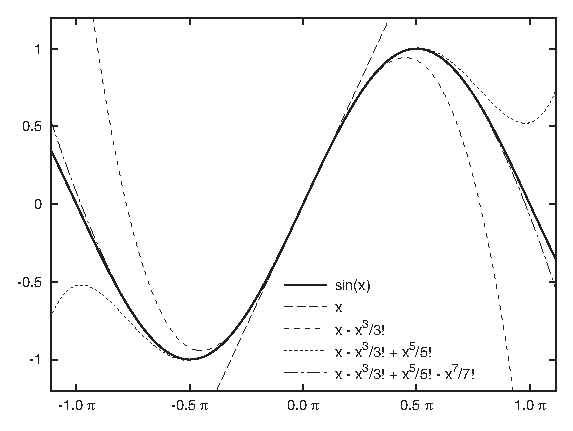
\includegraphics{img/taylorseries}}
  \caption{The sine function $\sin(x)$ and its Taylor expansions around
    zero, truncated after retaining different numbers of terms. If
    more terms are kept, the approximation is acceptable over a
    greater range of values.}
  \label{fig:taylorseries}\vspace*{-9pt}
\end{figure}

It is this last step that makes Taylor's theorem so useful from a
practical point of view: it tells us that \emph{we can approximate any
  smooth function locally by a polynomial}. And polynomials \index{polynomials!about} are always
easy to work with---often much easier than the complicated functions
that we started with.

One important practical point: the approximation provided by a
truncated Taylor series is good only \emph{locally}---that is, near
the point around which we expand. This is because in that case $x$ is
small (\ie, $x \ll 1$) and so higher powers become negligible fast.
Taylor series are usually represented in a form that assumes that the
expansion takes place around zero. If this is not the case, we need to
remove or factor out some large quantity so that we are left with a
``small parameter'' in which to expand. As an example, suppose we want to 
obtain an approximation to $e^x$ for values of $x$ near $10$.  If we
expanded in the usual fashion around zero, then we would have to sum
\emph{many} terms before\vadjust{\pagebreak} the approximation becomes good (the terms
grow until $10^n < n!$, which  means we need to keep more than 20
terms). Instead, we proceed as follows: we write $e^x  = e^{10 +
  \delta} = e^{10} \, e^{\delta} = e^{10} \,
(1+\delta+\frac{\delta^2}{2}+\dotsb)$. In other words, we set it up so
that $\delta$ is small allowing us to expand $e^{\delta}$ around zero
as before.

Another important point to keep in mind is that the function must be
smooth at the point around which we expand: it must not have a kink or
other singularity there. This is why the logarithm is usually expanded
around one (not zero): recall that the logarithm diverges as $x$ goes
to zero.

\begin{table}
\def\vrl{\smash{\vrule height96pt width.25pt depth4pt}}
\tbl{The first few terms of the Taylor expansion of some important
  functions\label{tbl:taylorseries}}{%
\begin{tabular}{c@{\hskip9pt}c@{\hskip9pt}l@{\hskip9pt}c@{\hskip9pt}c}\toprule
\TCH{Function} && \TCH{Taylor expansion} && \TCH{Comment}\\\colrule
$ e^x $ && $ 1 + x + \frac{x^2}{2!} + \frac{x^3}{3!} + \dotsb $ && all $x$ \\[3pt]
$ \sin x $ && $ x - \frac{x^3}{3!} + \frac{x^5}{5!} \mp \dotsb $ && all $x$ \\[3pt]
$ \cos x $ && $ 1 - \frac{x^2}{2!} + \frac{x^4}{4!} \mp \dotsb $ && all $x$ \\[3pt]
$ \log(1+x) $ && $ x - \frac{x^2}{2} + \frac{x^3}{3} \mp \dotsb $ &&
  $ -1 < x \le 1 $ \\[3pt]
$ \sqrt{1+x} $ && 
  $ 1 + \frac{x}{2} + \frac{x^2}{8} + \frac{x^3}{16} + \dotsb $ &&
  $ |x| \le 1 $ \\[3pt]
$ 1/(1+x) $ &\vrl& $ 1 - x + x^2 - x^3 \pm \dotsb $ &\vrl& $ |x| < 1 $ \\\botrule
\end{tabular}}
\end{table}

% ============================================================
\section{Useful Tricks}

% --------------------------------------------------  
\subsection{The Binomial Theorem}

\index{calculus!binomial theorem} 
\index{binomial theorem} 

Probably everyone has encountered the binomial formulas at some point:
%
\begin{gather*}
( a + b )^2 = a^2 + 2ab + b^2 \\
( a - b )^2 = a^2 - 2ab + b^2 
\end{gather*}
%
The binomial theorem provides an extension of this result to higher
powers. The theorem states that, for an arbitrary integer power $n$,
the expansion of the lefthand side can be written as:
%
\begin{align*}
( a + b )^n & = \sum_{k=0}^n \binom{n}{k} a^{n-k} b^k \\
            & = \binom{n}{0} a^n b^0 + \binom{n}{1} a^{n-1} b^1 
              + \binom{n}{2} a^{n-2} b^2 + \dots + \binom{n}{n} a^0 b^n
\end{align*}
%
This complicated-looking expression involves the
\emph{binomial coefficients}:
%
\[
\binom{n}{k} = \frac{n!}{k! \, (n-k)!} \qquad 0 \le k \le n
\]
%
The binomial coefficients are combinatorial factors that count the
number of different ways one can choose $k$ items from a set of $n$
items, and in fact there is a close relationship between the binomial
theorem and the binomial probability distribution.

As is the case for many exact results, the greatest practical use of
the binomial theorem comes from an approximate expression. Assume that
$b < a$, so that $b/a < 1$. Now we can write:
%
\begin{align*}
( a + b )^n & = a^n \paren{ 1 + \frac{b}{a} }^n \\
      & \approx a^n \paren{ 1 + n \frac{b}{a} 
                              + \frac{n(n-1)}{2} \paren{ \frac{b}{a} }^2
                              + \dotsb }
\end{align*}
%
Here we have neglected terms involving higher powers of $b/a$, which
are small compared to the retained terms, since $b/a < 1$ by
construction (so that higher powers of $b/a$, which involve
multiplying a small number repeatedly by itself, quickly become
negligible).

In this form, the binomial theorem is frequently useful as a way
to generate approximate expansions. In particular, the first-order
approximation:
%
\[
(1+x)^n \approx 1 + nx \qquad \text{for $|x| < 1$}
\]
%
should be memorized.


% --------------------------------------------------  
\subsection{The Linear Transformation}

\index{calculus!linear transformation} 
\index{linear transformation, calculus} 

Here is a quick, almost trivial, trick that is useful enough to be
committed to memory. Any variable can be transformed to a similar
variable that takes on only values from the interval $[0,1]$, via the
following linear transformation, where $x_{\text{\scriptsize min}}$ and
$x_{\text{\scriptsize max}}$ are the minimum and maximum values that $x$
can take on:
%
\[
y = \frac{x - x_{\text{\scriptsize min}}}{x_{\text{\scriptsize max}} - x_{\text{\scriptsize min}}}
\]
%
This transformation is frequently useful---for instance, if we have two
quantities and would like to compare how they develop over time. If
the two quantities have very different magnitudes, then we need to
reduce both of them to a common range of values. The transformation
just given does exactly that.

If we want the transformed quantity to \emph{fall} whenever the
original quantity goes up, we can do this by writing:
%
\[
\bar{y} = 1 - y = 1 - \frac{x - x_{\text{\scriptsize min}}}{x_{\text{\scriptsize max}} - x_{\text{\scriptsize min}}}
\]
%

We don't have to shift by $x_{\text{\scriptsize min}}$ and rescale by the original
range $x_{\text{\scriptsize max}} - x_{\text{\scriptsize min}}$. Instead, we can subtract any
``typical'' value and divide by any ``typical'' measure of the range.
In statistical applications, for example, it is frequently useful to
subtract the mean $\mu$ and to divide by the standard deviation
$\sigma$. The resulting quantity is referred to as the
\emph{$z$-score}:
%
\[
z = \frac{x-\mu}{\sigma}
\]
%
Alternatively, you might also subtract the median and divide by the
inter-quartile range. The exact choice of parameters is not crucial
and will depend on the specific application context. The important
takeaway here is that we can normalize any variable by:
\begin{itemize}
\item Subtracting a typical value (shifting) and
\item Dividing by the typical range (rescaling)
\end{itemize}

% --------------------------------------------------  
\subsection{Dividing by Zero}

\index{calculus!dividing by zero} 
\index{dividing by zero} 
\index{zero, dividing by} 

Please remember that \emph{you cannot divide by zero!} I am sure you
know this---but it's surprisingly easy to forget (until the computer
reminds us with a fatal ``divide by zero'' error).

It is instructive to understand what happens if you try to divide by
zero.  Take some fixed number (say, $1$), and divide it by a
sequence of numbers that approach zero:

\begin{align*}
\frac{1}{10}   & = 0.1 \\[3pt]
\frac{1}{5}    & = 0.2 \\[3pt]
\frac{1}{1}    & = 1.0 \\[3pt]
\frac{1}{1/5}  & = 5 \\[3pt]
\frac{1}{1/10} & = 10 \\[3pt]
\frac{1}{0}    & = \text{ ?}
\end{align*}

In other words, as you divide a constant by numbers that
\emph{approach} zero, the result becomes larger and larger. Finally,
if you let the divisor go to zero, the result grows beyond all bounds: it
diverges. Figure \ref{fig:zerodivisor} shows this graphically.

\begin{figure}
  \centerline{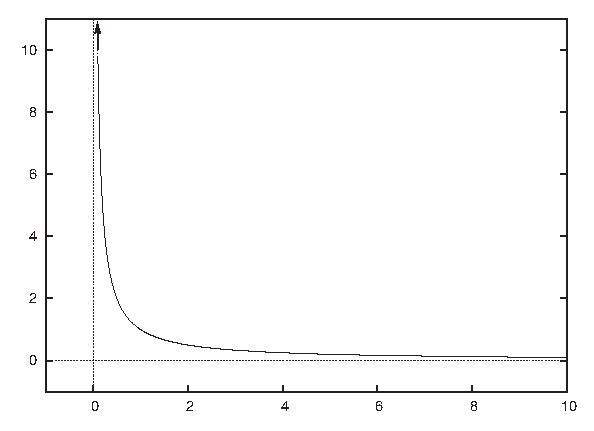
\includegraphics{img/zerodivisor}}
  \caption{As you divide a constant value by smaller and smaller
    numbers, the result is getting larger and larger. If you divide by
    zero, it blows up!}
  \label{fig:zerodivisor}
\end{figure}

What you should take away from this exercise and Figure
\ref{fig:zerodivisor} is that you cannot replace $1/0$ by something
else---for instance, it is \emph{not} a smart move to replace $1/0$ by
$0$ ``because both don't really mean anything, anyway.'' If you need
to find a numeric value for $1/0$, then it should be something like
``infinity,'' but this is not a useful value to operate with in
practical applications.

Therefore, \emph{whenever you encounter a fraction $\frac{a}{b}$ of
  any kind, \index{fractions!division by zero} you \emph{must} check whether the denominator can become
  zero and exclude these points from consideration}.

Failing to do so is one of the most common sources of error.  What is
worse, these errors are difficult to recover from---not just in
implementations but also\vadjust{\pagebreak} conceptually. A typical example involves
``relative errors,'' where we divide the difference between the
observed and the expected value by the expected value:
%
\[
\text{relative error} 
= \frac{\text{observed} - \text{expected}}{\text{expected}}
\]
%
What happens if for one day the expected value drops to zero?  You are
toast. There is no way to assign a meaningful value to the error in
this case. (If the observed value is also zero, then you can treat
this as a special case and \emph{define} the relative error to be zero
in this case, but if the observed value is not zero, then this
definition is obviously inappropriate.)

These kinds of problems have an unpleasant ability to sneak up on you.
A quantity such as the relative error or the defect rate (which is
also a ratio: the number of defects found divided by the number of
units produced) is a quantity commonly found in reports and
dashboards. You don't want your entire report to crash because no
units were produced for some product on this day rendering the
denominator zero in one of your formulas!

There are a couple of workarounds, neither of which is perfect. In the
case of the defect rate, where you can be sure that the numerator will
be zero if the denominator is (because no defects can be found if no
items were produced), you can add a small positive number to the
denominator and thereby prevent it from ever becoming exactly zero. As
long as this number is small compared to the number of items typically
produced in a day, it will not significantly affect the reported
defect rate, but will relieve you from having to check for the
$\frac{0}{0}$ special case explicitly. In the case of calculating a
relative error, you might want to replace the numerator with the
average of the expected and the observed values. The advantage is that
now the denominator can be zero only\vadjust{\pagebreak} if the numerator is zero, which
brings us back to the suggestion for dealing with defect rates just
discussed. The problem with this method is that when no events are
observed but some number was expected, the relative error is reported
as $-2$ (negative 200~percent instead of negative 100~percent); this is due to the
factor $1/2$ in the denominator, which comes from calculating the
average there.

So, let me say it again: whenever you are dealing with fractions, you
\emph{must} consider the case of denominators becoming zero.  Either
rule them out or handle them explicitly.

% ============================================================
\section{Notation and Basic Math}

\index{calculus!mathematical notation|(} 
\index{mathematics!notation|(} 

This section is not intended as a comprehensive overview of
mathematical notation or as your first introduction to mathematical
formulas. Rather, it should serve as a general reminder of some basic
facts and to clarify some conventions used in this book. (All my
conventions are pretty standard---I have been careful not to use any
symbols or conventions that are not generally used and understood.)

% --------------------------------------------------  
\subsection{On Reading Formulas}

\index{formulas} 

A mathematical formula combines different components, called
\emph{terms}, by use of operators. The most basic operators are
\emph{plus} and \emph{minus} ($+$ and $-$) and \emph{multiplied by}
and \emph{divided by}\break ($\cdot$ and $/$). Plus and minus are always
written explicitly, but the multiplication operator is usually
silent---in other words, if you see two terms next to each other, with
nothing between them, they should be multiplied. The division operator
can be written in two forms: $1/n$ or $\frac{1}{n}$, which mean
exactly the same thing. The former is more convenient in text such as
this; the latter is more clear for long, ``display'' equations. An
expression such as $1/n + 1$ is ambiguous and should not be used, but
if you encounter it, you should assume that it means $\frac{1}{n} + 1$
and not $1/(n+1)$ (which is equivalent to $\frac{1}{n+1}$).

Multiplication and division have higher precedence than addition and
subtraction, therefore $a b + c$ means that first you multiply $a$ and
$b$ and then add $c$ to the result.  To change the priority, you need
to use parentheses: $a (b+c)$ means that first you add $b$ and $c$ and
then multiply the result by $a$. Parentheses can either be round
$(\dots)$ or square $[\dots]$, but their meaning is the same.

Functions take one (or several) arguments and return a result. A
function always has a \emph{name} followed by the \emph{arguments}.
Usually the arguments are enclosed in parentheses: $f(x)$. Strictly
speaking, this notation is ambiguous because an expression such as
$f(a+b)$ could mean either ``add $a$ and $b$ and then multiply by
$f$'' or ``add $a$ and $b$ and then pass the result to the function
$f$.'' However, the meaning is usually clear from the context.

(There is a slightly more advanced way to look at this. You can think
of $f$ as an operator, similar to a differential operator like
$\frac{\rm d}{{\rm d} x}$ or an integral operator like $\int
\text{d}t$. This operator is now\vadjust{\pagebreak} applied to the expression to the
right of it. If $f$ is a function, this means applying the function to
the argument; if the operator is a differential operator, this means
taking the derivative; and if $f$ is merely a number, then applying it
simply means multiplying the term on its right by it.)

A function may take more than one argument; for example, the function
$f(x,y,z)$ takes three arguments. Sometimes you may want to emphasize
that not all of these arguments are equivalent: some are actual
variables, whereas others are ``parameters,'' which are kept constant
while the variables change. Consider $f(x) = a x + b$. In this
function, $x$ is the variable (the quantity usually plotted along the
horizontal axis) while $a$ and $b$ would be considered parameters.  If
we want to express that the function $f$ does depend on the parameters
as well as on the actual variable, we can do this by including the
parameters in the list of arguments: $f(x,a,b)$. To visually separate
the parameters from the actual variable (or variables), a semicolon is
sometimes used: $f(x;a,b)$.  There are no hard-and-fast rules for when
to use a semicolon instead of a comma---it's simply a convenience that
is sometimes used and other times not.

One more word on functions: several functions are regarded as ``well
known'' in mathematics (such as sine and cosine, the exponential
function, and the logarithm). The names of such well-known functions
are always written in upright letters, whereas functions in general
are denoted by an italic letter.  (Variables are always written in
italics.) For well-known functions, the parentheses around the
arguments can be omitted if the argument is sufficiently simple. (This
is another example of the ``operator'' point of view mentioned
earlier.) Thus we may write $\sin(x+1) + \log x - f(x)$ (note the
upright letters for sine and logarithm, and the parentheses around the
argument for the logarithm have been omitted, because it consists of
only a single term).  This has a different meaning than: $\sin(x+1) +
\log( x - f(x) )$.

% --------------------------------------------------  
\subsection{Elementary Algebra}

\index{algebra!about} 

For numbers, the following is generally true:
%
\[
a ( b + c ) = a b + a c
\]
%
This is often applied in situations like the following, where we
\emph{factor out} the $a$:
%
\[
a + b = a( 1 + b/a ) 
\]
%
If $a$ is much greater than $b$, then we have now converted the
original expression $a + b$ into another expression of the form:
%
\[
\text{\textit{something large}} \cdot (1 + \text{\textit{something small}})
\]
%
which makes it easy to see which terms matter and which can be
neglected in an approximation scheme. (The small term in the
parentheses is ``small'' compared to the $1$ in the parentheses and
can therefore be treated as a perturbation.)

Quantities can be multiplied together, which gives rise to
\emph{powers}:
%
\begin{gather*}
a \cdot a = a^2 \\
a \cdot a \cdot a = a^3 \\
\dots
\end{gather*}
%
The raised quantity (the superscript) is also referred to as the
\emph{exponent}. In this book, superscripts always denote powers. 

The three binomial formulas should be committed to memory:
%
\begin{gather*}
( a + b )^2 = a^2 + 2ab + b^2 \\
( a - b )^2 = a^2 - 2ab + b^2 \\
( a + b ) ( a - b ) = a^2 - b^2
\end{gather*}
%
Because the easiest things are often the most readily forgotten,
let me just work out the first of these identities explicitly:
%
\begin{align*}
( a + b )^2 
& = ( a + b ) ( a + b ) \\
& = a ( a + b ) + b ( a + b ) \\
& = a^2 + a b + b a + b^2 \\
& = a^2 + 2 a b + b^2 
\end{align*}
%
where I have made use of the fact that $a b = b a$.

\subsection{Working with Fractions}

\index{fractions!about} 

Let's review the basic rules for working with fractions. The
expression on top is called the \emph{numerator}, the one at the
bottom is the \emph{denominator}:
%
\[
\frac{\text{numerator}}{\text{denominator}}
\]
%

If you can factor out a common factor in both numerator and
denominator, then this common factor can be canceled:
%
\[
\frac{2 + 4x}{2 + 2\sin(y)} 
= \frac{2 (1+2x)}{2(1+\sin(y)} = \frac{ 1 + 2 x }{ 1 + \sin y} 
\]
%

To add two fractions, you have to bring them onto a common denominator
in an operation that is the opposite of canceling a common factor:
%
\[
\frac{1}{a} + \frac{1}{b} = \frac{a}{ab} + \frac{b}{ab} = \frac{a+b}{ab}
\]
%
Here is a numeric example:
%
\[
\frac{1}{2} + \frac{1}{3} = \frac{3}{6} + \frac{2}{6} = \frac{5}{6}
\]
%

% --------------------------------------------------  
\subsection{Sets, Sequences, and Series}

\index{sets, sequences and series} 

A \emph{set} is a grouping of elements in no particular order.  In a
\emph{sequence}, the elements occur in a fixed order, one after the
other.

The individual elements of sets and sequences are usually shown with
subscripts that denote the index of the element in the set or its
position in the sequence (similar to indexing into an array). In this
book, subscripts are used only for the purpose of indexing elements of
sets or sequences in this way.

Sets are usually indicated by curly braces. The following expressions
are equivalent:
\begin{gather*}
\braces{ x_1, x_2, x_3, \dots, x_n } \\
\braces{ x_i \: | \; i = 1, \dots, n }
\end{gather*}

For brevity, it is customary to suppress the range of the index if it
can be understood from context. For example, if it is clear that there
are $n$ elements in the set, I might simply write $\braces{x_i}$.

One often wants to sum a finite or infinite sequence of numbers; the
result is known as a \emph{series}:
%
\[
x_1 + x_2 + x_3 + \dots + x_n
\]
%
Instead of writing out the terms explicitly, it is often useful to
use the sum notation:
%
\[
\sum_{i=1}^n x_i = x_1 + x_2 + x_3 + \dots + x_n
\]
%

The meaning of the summation symbol should be clear from this example.
The variable used as index (here, $i$) is written underneath the
summation sign followed by the lower limit (here, $1$).  The upper
limit (here, $n$) is written above the summation sign.  As a
shorthand, any one of these specifications can be omitted. For
instance, if it is clear from the context that the lower limit is $1$
and the upper limit is $n$, then I might simply write $\sum_i x_i$ or
even $\sum x_i$. In the latter form, it is understood that the sum runs
over the index of the summands.

It is often convenient to describe the terms to be summed over in
words, rather than giving specific limits:
%
\[
\sum_{\rm{all\  data\  points}} x_i
\]
%

Some standard transformations involving the summation notation are
used fairly often. For example, one frequently needs to shift indices.
The following three expressions are equal, as you can easily see by
writing out explicitly the terms of the sum in each case:
%
\[
\sum_{i=0}^n x_i = \sum_{i=1}^{n+1} x_{i-1} = x_0 + \sum_{i=1}^n x_i
\]
%
Keep in mind that the summation notation is just a shorthand for
the explicit form given at the start of this section. If you become
confused, you can always write out the terms explicitly to understand
what is going on.

Finally, we may take the upper limit of the sum to be infinity, in
which case the sum runs over infinitely many terms. Infinite series
play a fundamental role in the theoretical development of mathematics,
but all series that you will encounter in applications are, of course,
finite.

% --------------------------------------------------  
\subsection{Special Symbols}

\index{symbols|(} 
\index{special symbols|(} 

A few mathematical symbols are either indispensable or so useful that
I wouldn't do without them.

\subsubsection{Binary relationships}

\index{binary relationships}
 
There are several special symbols to describe the relationship between
two expressions. Some of the most useful ones are listed in Table
\ref{tbl:relops}.

\begin{table}[h]
\def\vrl{\smash{\vrule height86pt width.25pt depth5pt}}
\tbl{Commonly used relational operators\label{tbl:relops}}{%
\begin{tabular}{c@{\hskip9pt}c@{\hskip9pt}l}
\toprule
\TCH{Operator} && \TCH{Meaning}\\
\colrule
$=$ $\ne$   && equal to, not equal to  \\
$<$ $>$     && less than, greater than \\
$\le$ $\ge$ & &less than or equal to, greater than or equal to \\[2pt]
$\ll$ $\gg$ && much less than, much greater than \\
$\propto$   && proportional to \\
$\approx$   && approximately equal to \\
$\sim$      &\vrl& scales as \\
\botrule
\end{tabular}}
\end{table}

The last three might require a word of explanation. We say two
quantities are \emph{approximately equal} when they are equal up to a
``small'' error. Put differently, the difference between the two
quantities must be small compared to the quantities themselves: $x$
and $1.1 x$ are approximately equal, $x \approx 1.1 x$, because
the difference (which is $0.1 x$) is small compared to $x$.

One quantity is \emph{proportional} to another if they are equal
up to a constant factor that has been omitted from the expression.
Often, this factor will have units associated with it. For
example, when we say ``time is money,'' what we really mean is:
%
\[
\text{money} \propto \text{time}
\]
%
Here the omitted constant of proportionality is the hourly rate (which
is also required to fix the units: hours on the left, dollars on the
right; hence hourly rate must have units of ``dollars per hour'' to
make the equation dimensionally consistent).

We say that a quantity \emph{scales as} some other quantity if we want
to express how one quantity depends on another one in a very general
way. For example, recall that the area of a circle is $\pi r^2$ (where
$r$ is the length of the radius) but that the area of a square is
$a^2$ (where $a$ is the length of the side of the square). We can now
say that ``the area \emph{scales as} the square of the length.''  This
is a more general statement than saying that the area is proportional
to the square of the length: the latter implies that they are equal up
to a constant factor, whereas the scaling behavior allows for more
complicated dependencies. (In this example, the constant of
proportionality depends on the \emph{shape} of the figure, but the
scaling behavior $\text{area} \sim \text{length}^2$ is true for all
symmetrical figures.)

In particular when evaluating the complexity of algorithms, there is
another notation to express a very similar notion: the so-called
\emph{big O} notation. For example, the expression $\mathcal{O}(n^2)$
states that the complexity of an algorithm grows (``scales'') with the
square of the number of elements in the input.

\subsubsection{Parentheses and other delimiters}

\index{parenthesis and other delimiters} 
\index{delimiters} 

Round parentheses $\paren{\dots}$ are used for two purposes: to group
terms together (establishing precedence) and to indicate the arguments
to a function: 
%
\begin{align*}
& a b + c \ne a (b + c) & & \text{Parentheses to establish precedence} \\
& f(x,y) = x + y        & & \text{Parentheses to indicate function arguments}
\end{align*}
%

Square brackets $\brackets{\dots}$ are mostly used to indicate an
interval:
%
\[
[a,b] \qquad \text{all $x$ such that $a \le x \le b$}
\]
%
For the purpose of this book, we don't need to worry about the
distinction between closed and open intervals (\ie, intervals that do
or don't contain their endpoints, respectively).

Very rarely I use brackets for other purposes---for example as an
alternative to round parentheses to establish precedence, or indicate
that a function takes another \emph{function} as its argument, as in
the expectation value: $E[ f(x) ]$.

Curly braces $\braces{\dots}$ always denote a set.


\subsubsection{Miscellaneous symbols}

Two particular constants are indispensable.  Everybody has heard of
$\pi = 3.141592\dots$, which is the ratio of the circumference of a
circle to its diameter:
%
\[
\pi = \frac{\text{circumference}}{\text{diameter}} = 3.141592\dots
\]

Equally important is the ``base of the natural logarithm'' $e =
2.718281\dots$, sometimes called Euler's number.\index{base of the natural logarithm}\index{Euler's number}\index{e@$e$ (base of the natural logarithm} It is defined as the
value of the infinite series:
%
\[
e = \sum_{n=0}^\infty \frac{1}{n!} = 2.718281\dots
\]
%
The function $e^x$ obtained by raising $e$ to the $x$th power has the
property that its derivative also equals $e^x$, and it is the only
function that equals its derivative (up to a multiplicative constant,
to be precise).

The number $e$ also shows up in the definition of the Gaussian 
function:
%
\[
e^{-x^2}
\]
%
(Any function that contains $e$ raised to $- x^2$ power is called a
``Gaussian''; \index{Gaussian distribution (Gaussian function)!e raised@$e$ raised to $- x^2$ power} what's crucial is that the $x$ in the exponent is
squared and enters with a negative sign. Other constants may appear
also, but the $-x^2$ in the exponent is the defining property.)

Because the exponents are often complicated expressions themselves,
there is an alternative notation for the exponential function that
avoids superscripts and instead uses the function name $\exp(\dots)$.
The expression $\exp(x)$ means exactly the same as $e^x$, and the
following two expressions are equivalent, also---but the one on the
right is easier to write:
%
\[
e^{-\paren{ \frac{x-\mu}{\sigma} }^2 } 
= \exp \paren{-\paren{ \frac{x-\mu}{\sigma} }^2 } 
\]

A value of infinite magnitude is indicated by a special symbol:
%
\[
\infty \qquad \text{a value of infinite magnitude}
\]

The square root sign $\sqrt{x}$ states that:
%
\[
\text{if $\quad y = \sqrt{x} \quad $ then $\quad y^2 = x$}
\]

Finally, the integral sign $\int$, which always occurs together with
an expression of the form $\text{d}x$ (or $\text{d}t$, or so), is used
to denote a generalized form of summation: the expression to the right
of the integral sign is to be ``summed'' for all values of $x$ (or
$t$). If explicit limits of the integration are given, they are
attached to the integral sign:
%
\[
\int_0^1 f(x) \rms{x}
\]
%
This means: ``sum all values of $f(x)$ for $x$ ranging from $0$ to
$1$.''

\index{symbols|)} 
\index{special symbols|)} 

% --------------------------------------------------    
\subsection{The Greek Alphabet}

\index{Greek alphabet} 

Greek letters are used all the time in mathematics and other sciences
and should be committed to memory. (See Table \ref{tbl:greek}.)

\begin{table}[h]
\tbl{The Greek alphabet\label{tbl:greek}}{%
\begin{tabular}{c@{\hskip9pt}c@{\hskip9pt}c@{\hskip9pt}c@{\hskip9pt}l}
\toprule
\TCH{Lowercase} && \TCH{Uppercase} && \TCH{Name} \\\colrule
$ \alpha $ && $ A     $  && Alpha \\
$ \beta $  && $ B     $  && Beta \\
$ \gamma $ && $ \Gamma $ && Gamma \\
$ \delta $ && $ \Delta $ && Delta \\
$ \epsilon $ && $ E    $ && Epsilon \\
$ \zeta $  && $ Z     $  && Zeta \\
$ \eta $   && $ H     $  && Eta \\
$ \theta $ && $ \Theta $ && Theta \\
$ \iota $  && $ I     $  && Iota \\
$ \kappa $ && $ K     $  && Kappa \\
$ \lambda $ && $ \Lambda $ && Lambda \\
$ \mu $    && $ M   $    && Mu \\
$ \nu $    && $ N   $    && Nu \\
$ \xi $    && $ \Xi $    && Xi \\
$ o      $ && $ O $      && Omicron \\
$ \pi $    && $ \Pi $    && Pi \\
$ \rho $   && $ R    $   && Rho \\
$ \sigma $ && $ \Sigma $ && Sigma \\
$ \tau $   && $ T    $   && Tau \\
$ \upsilon $ && $ \Upsilon $ && Upsilon \\
$ \phi $   && $ \Phi $   && Phi \\
$ \chi $   && $ X $      && Chi \\
$ \psi $   && $ \Psi $   && Psi \\
$ \omega $ && $ \Omega $ && Omega \\\botrule
\end{tabular}}\vspace*{-9pt}
\end{table}
 
\index{calculus!mathematical notation|)} 
\index{mathematics!notation|)} 
 
% ============================================================
\section{Where to Go from Here}

This appendix can of course only give a cartoon version of the topics
mentioned, or---if you have seen this material before---at best serve
as a reminder.  But most of all, I hope it serves as a \emph{teaser}:
mathematics is a wonderfully rich and stimulating topic, and I would
hope that in this appendix (and in the rest of this book) I have been
able to convey some of its fascination---and perhaps even convinced
you to dig a little deeper.

If you want to learn more, here are a couple of hints.

The first topic to explore is calculus (or real analysis). All modern
mathematics starts here, and it is here that some of the most
frequently used concepts (derivative, integral, Taylor expansion) are
properly introduced. It is a must-have.

But if you limit your attention to calculus, you will never get
over the idea that mathematics is about ``calculating something.'' To
get a sense of what math is \emph{really} all about, you have to go
beyond analysis. The next topic in a typical college syllabus is
linear algebra.  In linear algebra, we go beyond relatively tangible
things like curves and numbers and for the first time start to
consider concepts in a fully abstract way: spaces, transformations,
mappings.  What can we say\vadjust{\pagebreak} about them \emph{in general} without having
to appeal to any particular realization? Understanding this material
requires real mental effort---you have to change the way you think.
(Similarly to how  you have to change the way you think if you try to
learn Lisp or Haskell.) Linear algebra also provides the theoretical
underpinnings of all matrix operations and hence for most
frequently used numerical routines. (You can't do paper-and-pencil
mathematics without calculus, and you can't do numerical mathematics
without linear algebra.)

With these two subjects under your belt, you will be able to pick up
pretty much any mathematical topic and make sense of it.  You might
then want to explore complex calculus for the elegance and beauty of
its theorems, or functional analysis and Fourier theory (which blend
analysis and linear algebra) because of their importance in all
application-oriented areas, or take a deeper look at probability
theory, with its obvious importance for anything having to do with
random data.

\subsection{On Math}

\index{calculus!on math} 

I have observed that there are two misconceptions about mathematics
that are particularly prevalent among people coming from a software or
computing background.  The first misconception holds that mathematics
is primarily a prescriptive, calculational (not necessarily numerical)
scheme and similar to an Algol-derived programming language: a
pseudo-code for expressing algorithms.  The other misconception views
mathematics as mostly an abstract method for formal reasoning, not
dissimilar to certain logic programming environments: a way to
manipulate logic statements.

What both of them miss is that mathematics is not a \emph{method} but
first and foremost a body of \emph{content} in its own right. You will
never understand what mathematics is if you see it only as something
you \emph{use} to obtain certain results. Mathematics is, first and
foremost, a rich and exciting story in itself.

There is an unfortunate perception among nonmathematicians (and even
partially reinforced by this book) that mathematics is about
``calculating things.'' This is not so, and it is probably the most
unhelpful misconception about mathematics of all.

In fairness, this point of view is promulgated by many introductory
college textbooks. In a thoroughly misguided attempt to make their
subject ``interesting,'' they try to motivate mathematical concepts
with phony applications to the design of bridges and airplanes, or to
calculating the probability of winning at poker. This not only
obscures the beauty of the subject but also creates the incorrect
impression of mathematics as a utilitarian fingering exercise and
almost as a necessary evil.

Finally, I strongly recommend that you stay away from books on popular
or recreational math, for two reasons. First, they tend to focus on a
small set of topics that can be treated using ``elementary'' methods
(mostly geometry and some basic number theory), and tend to omit most
of the conceptually important\vadjust{\pagebreak} topics.  Furthermore, in their attempt
to present amusing or entertaining snippets of information, they fail
to display the rich, interconnected structure of mathematical theory:
all you end up with is a book of (stale) jokes.\vspace*{-6pt}


% ============================================================
\section{Further Reading}

\subsection{Calculus}

\begin{itemize}
\item \cit{The Hitchhiker's Guide to Calculus}{Michael
    Spivak}{Mathematical Association of America}{1995}
  If the material in this appendix is really new to you, then
  this short (120-page) booklet provides a surprisingly complete,
  approachable, yet mathematically respectable introduction. Highly
  recommended for the curious and the confused.

\item \cit{Precalculus: A Prelude to Calculus}{Sheldon
    Axler}{Wiley}{2008}
  Axler's book covers the basics: numbers, basic algebra,
  inequalities, coordinate systems, and functions---including
  exponential, logarithmic, and trigonometric functions---but it stops
  short of derivatives and integrals. If you want to brush up on
  foundational material, this is an excellent text.

\item \cit{Calculus}{Michael Spivak}{4th ed., Publish or Perish}{2008}
  This is a comprehensive book on calculus. It concentrates
  exclusively on the clear development of the mathematical theory and
  thereby avoids the confusion that often results from an oversupply
  of (more or less) artificial examples. The presentation is written
  for the reader who is relatively new to formal mathematical
  reasoning, and the author does a good job motivating the peculiar
  arguments required by formal mathematical manipulations. Rightly
  popular.

\item \cit{Yet Another Introduction to Analysis}{Victor
    Bryant}{Cambridge University Press}{1990}
  This short book is intended as a quick introduction for those
  readers who already possess passing familiarity with the topic and
  are comfortable with abstract operations.
\end{itemize}

\vspace*{-6pt}
\subsection{Linear Algebra}

\begin{itemize}
\item \cit{Linear Algebra Done Right}{Sheldon Axler}{2nd ed.,
    Springer}{2004}
  This is the best introduction to linear algebra that I am aware of,
  and it fully lives up to its grandiose title. This book treats
  linear algebra as abstract theory of mappings, but on a very
  accessible, advanced undergraduate level. Highly recommended.

\item \cit{Linear Algebra}{Klaus J\"anich}{Springer}{1994}
  This book employs a greater amount of abstract mathematical
  formalism than the previous entry, but the author tries very hard to
  explain and motivate all concepts. This book might therefore give a
  better sense of the nature of abstract algebraic arguments than
  Axler's streamlined presentation. The book is written for a 
first-year course at German universities; the style of the presentation
  may appear exotic to the American reader.
\end{itemize}
 

\subsection{Complex Analysis}

%   It has been said that any book on complex variables is good, and 
%   there is some truth to that: the material is very regular and totally
%   understood, making it easy to write accessible books. 

\begin{itemize}
\item \cit{Complex Analysis}{Joseph Bak and Donald J.\ Newman}{2nd
    ed., Springer}{1996}
  This is a straightforward, and relatively short, introduction to all
  the standard topics of classical complex analysis. 

\item \cit{Complex Variables}{Mark J.\ Ablowitz and Athanassios S.\
    Fokas}{2nd ed., Cambridge University Press}{2003}
  This is a much more comprehensive and advanced book. It is split into
  two parts: the first part developing the theory, the second part
  discussing several nontrivial applications (mostly to the theory of
  differential equations).

\item \cit{Fourier Analysis and Its Applications}{Gerald B.\
    Folland}{American Mathematical Society}{2009}
  This is a terrific introduction to Fourier theory. The book places a
  strong emphasis on the solution of partial differential equations
  but in the course of it also develops the basics of function spaces,
  orthogonal polynomials, and eigenfunction expansions. The later
  chapters give an introduction to distributions and Green's
  functions.  This is a very accessible book, but you will need a
  strong grounding in real and complex analysis, as well as some
  linear algebra.
\end{itemize}

\subsection{Mindbenders}

If you \emph{really} want to know what math is like, pick up any one
of these. You don't have to understand everything---just get the
flavor of it all. None of them are ``useful,'' all are fascinating.

\begin{itemize}
\item \cit{A Primer of Analytic Number Theory}{Jeffrey
    Stopple}{Cambridge University Press}{2003}
  This is an amazing book in every respect. The author takes one of
  the most advanced, obscure, and ``useless'' topics---namely analytic
  number theory---and makes it completely accessible to anyone having
  even minimal familiarity with calculus concepts (and even those are
  not strictly required). In the course of the book, the author
  introduces series expansions, complex numbers, and many results from
  calculus, finally arriving at one of the great unsolved problems in
  mathematics: the Riemann hypothesis.  If you want to know what math
  \emph{really} is, read this book!

\item \cit{The Computer As Crucible: An Introduction to Experimental
    Mathematics}{Jonathan Borwein and Keith Devlin}{AK Peters}{2008}
  If you are coming from a programming background, you might be
  comfortable with this book. The idea behind ``experimental
  mathematics'' is to see whether we can use a computer to provide us
  with intuition about mathematical results that can later be verified
  through rigorous proofs. Some of the observations one encounters in
  the process are astounding. This book tries to maintain an
  elementary level of treatment.

\item \cit{Mathematics by Experiment}{Jonathan M.\ Borwein and David
    H.\ Bailey}{2nd ed., AK Peters}{2008}
  This is a more advanced book coauthored by one of the authors of the
  previous entry on much the same topic.

\item \cit{A Mathematician's Lament: How School Cheats Us Out of Our
    Most Fascinating and Imaginative Art Form}{Paul Lockhart}{Bellevue
    Literary Press}{2009}
  This is not a math book at all: instead it is a short essay by a
  mathematician (or math teacher) on \emph{what} mathematics is and
  \emph{why} and \emph{how} it should be taught.  The author's
  philosophy is similar to the one I've tried to present in the
  observations toward the end of this appendix. Read it and weep.
  (Then go change the world.) Versions are also available on the Web
  (for example, check
  \url{http://www.maa.org/devlin/devlin}\_\url{03}\_\url{08.}\break \url{html}).
\end{itemize}

\index{data analysis!calculus|)} 
\index{calculus|)} 
\clearpage
\
\thispagestyle{empty}
\
\clearpage